\section{Experiments}\label{sec:experiments}
Experiments are conducted in this section in order to answer the following research questions:
\begin{itemize}
    \item \textbf{RQ1}: Does CSGCN outperform state-of-the-art methods for the task of context-aware list prediction?
    \item \textbf{RQ2}: Can CSGCN be used to make non-context specific recommendations through aggregations?
    \item \textbf{RQ3}: Does side-information improve results for context-aware recommendations?
\end{itemize}
% \begin{itemize}
%     \item Datasets
%     \item Metrics
%     \item Problems with evaluation with context
%     \item Hyperparameter tuning
%     \item Other methods
%     \item Ablation study?
% \end{itemize}

\subsection{Experimental Settings}
\begin{adjustwidth}{-2.5 cm}{-2.5 cm}\centering
\begin{threeparttable}[!htb]
\caption{Statistics of the datasets.}\label{tab:datasetstats}
\scriptsize
\begin{tabular}{lrrrrrr}\toprule
\textbf{Dataset} &\textbf{User \#} &\textbf{Item \#} &\textbf{Interaction \#} &\textbf{Context \#} &\textbf{Sideinfo \#} \\\cmidrule{1-6}
ML1m &6,040 &3,377 &999,416 &4 &4 \\\cmidrule{1-6}
%ML100k &943 &1,682 &100,000 &4 &4 \\\cmidrule{1-6}
Frappe &546 & 821 &85,541 &2 &4 \\\cmidrule{1-6}
Yelp-NC &2,274 &2,140 &130,627 &4 &4 \\\cmidrule{1-6}
Yelp-ON &5,185 &5,566 &332,291 &4 &4 \\\midrule
\bottomrule
\end{tabular}
\end{threeparttable}
\end{adjustwidth}
%Ml1M og ML100k side info:  (age, gender, occupation, zipcode, genre)
%ML1M og ML100k context: (weekday, time of day)
%Frappe side info: (cost, city)
%Frappe context: (weekday, time of day, is weekend, weather)
%Yelp sideinfo: (genre, yelping since, fans, average stars) 
%Yelp context: (month, day_of_week, hour, timeofday)
%YelpNC categories: 80
%YelpOH categories: 75
To test the model on datasets with varying sizes and density, the following datasets were chosen:\\
%\textbf{MovieLens 100k (ML100k)} is a relatively small and dense dataset with 100.000 interactions between 943 users and 1,682 items.\\
\textbf{MovieLens 1M (ML1M)} is a dataset with 1 million interactions between 6,040 users and 3,377 movies.\\
It has the following side-information for users:
\begin{itemize}
    \item Age
    \item Gender
    \item Occupation
    \item Zipcode
\end{itemize}
Side-information for items is \textit{genre}, which specifies that an item has zero or more of the 18 genres available in the dataset.
For contextual information, the MovieLens datasets provide a timestamp for when the interaction took place, which is split into a month, day of week, hour and time of day (morning, evening, night, etc.).\\\\

The two Yelp datasets (\textbf{Yelp-NC} and \textbf{Yelp-ON}) are subsets of the public Yelp datasets, where we take the subset of items located in respectively North Carolina (NC) and Ontario (ON).
Both Yelp datasets have been pruned such that only users with at least 10 interactions, such that we can generate a stratified datasplit and avoid cold-start situations.\\
They both have the following side-information about users:
\begin{itemize}
    \item Yelping since (Year)
    \item Number of fans
    \item Average stars 
\end{itemize}
As with the MovieLens dataset, the side-information about items a feature specifying the categories that an item belongs to.
For the YelpNC dataset, this is zero or more of 80 different categories, and 75 categories for YelpON.\\
The contextual information is a timestamp, which is split into four types as with the MovieLens dataset.\\
Finally, the \textbf{Frappe} dataset contains information about how users have interacted with applications on their smartphones.
The only available side-information for users here is their city, and for items whether the application is free or not.
However, it contains contextual information about the time of the transaction:
\begin{itemize}
    \item Weekday
    \item Time of day
    \item Whether it is weekend or not
\end{itemize}
It also contains information about the weather at the time of the transaction.

\subsection{Feature selection}
Since most of the datasets mainly include a timestamp as contextual information, we discretize these into the following features:
\begin{itemize}
	\item Month
	\item Day of week
	\item Hour
	\item Time of day
\end{itemize}
Time of day is a further discretization of the hour feature, split into 5 intervals:
\begin{itemize}
	\item Night (0 to 4)
	\item Morning (4 to 8)
	\item Before midday (8 to 12)
	\item After midday (12 to 16)
	\item Afternoon (16 to 20)
	\item Late night (20 to 24)
\end{itemize}
For the Frappe dataset, we instead make use of the three default contextual values available (weekday, time of day, weekend or not).
\\\\
For the side-information, we use all the available side-information for both users and items with some discretization.
The Yelp datasets provide a "yelping since" feature, which is a timestamp for the creation of the user.
This is discretized to include the year that the user has been created.
\\
Additionally, the feature "fans" is discretized into four groups:
\begin{itemize}
	\item $< 50$ fans
	\item $50 - 100$ fans
	\item $100-500$ fans
	\item $> 500$ fans
\end{itemize}


\subsection{Parameter settings}
To fairly compare the performance of the models, we train all of them by optimizing the BPR loss with Adam.
The learning rate is searched between $[0.1, 0.01, 0.001, 0.0001]$ for all models.
The batch size is set as 1024 for all datasets except Frappe, where it is set to 512 due to its size.
The embedding size is set to 64, and for the models using regularization terms, this is searched between $[0.01, 0.001, 0.0001]$.
For CFM and NFM we follow the approach presented in the original papers and feed them with a pretrained FM model which has run for 500 epochs with the settings presented in the CFM paper.
Since we do not utilize multi-hot, the multi-hot attention mechanism of CFM is disabled as described in their paper.
All methods are run for a max of 1000 epochs with an early stopping mechanism triggered when the HR@20 or Recall@20 has not improved for 5 steps.


\subsection{Evaluation Types \& Metrics}\label{subsec:evalandmetrics}
The objective of the models in the experiments is to produce a top-$k$ list of items for a user. 
Different methods for evaluating the performance of the models were considered, specifically the fold-out and leave-one-out methods.
These methods interact with the context in different ways.
For the fold-out method, the datasets are split into a training set and a test set, where the model is trained on the training set and evaluated on the test set. 
This split is generated such that each user in the test set is also found in the training set.
Using this stratified split method, we decided to use a split of 80\% training and 20\% test split.
Because of this split, a single user can have multiple ground truth entries across multiple contexts.\\
A problem to consider with fold-out for content-aware evaluation is that when context is a part of the input to the model, a score must be calculated for each combination of item and context due to the multiple ground truth contexts, which can be quite computationally expensive.
A single context cannot be guaranteed for the user, and thus every context needs to be evaluated.
\\\\
For the leave-one-out method, the newest interaction for each user is removed from the training and used a as test set, as per \cite{CFM, BPR}.
This means that when a top-$k$ list is produced for a user, only a single item amongst the recommended items can be relevant, and thus there is only one context within which the ground truth was made.
This approach is largely inspired by sequential recommendation systems, where you leave out the newest interaction from each user and try to predict it based on the sequence of the previous interactions by the user.\\
This approach limits the number of different metrics that can be used for this type of evaluation method, and it tends to report worse results than the fold-out method.
\\\\
For comparisons, we conduct an experiment using fold-out for models that produce a top-$k$ recommendation list, and conduct a separate leave-one-out evaluation for models that produce a context-aware top-$k$ recommendation list. 
The metrics used for the fold-out evaluation are Precision@N, Recall@N and NDCG@N, while the leave-one-out experiments report HR@N and MRR@N.
\\\\
The top-$k$ recommendation problem is the task of recommending a list $L(u)$ to an active user $u$ containing $k$ items to likely be of interest.
Evaluating the quality of such a method can be done by splitting the set of items $I$ into a training set $I_{train}$ used to learn $L$ and a test set $I_{test}$ for each user $u$.
\\
Let $T(u) \subset I_u \cap I_{test}$, where $I_u$ is the subset of items that have been interacted with by user $u$, then precision can be calculated according to \Cref{eqn:precision}, and recall according to \Cref{eqn:recall}.
Precision defines the proportion of relevant instances among the predicted relevant items, while recall is the proportion of true positives that were correctly predicted.
\begin{equation}
    \label{eqn:precision}
    Precision@N(L) = \frac{1}{|U|} \sum\limits_{u \epsilon U}\frac{|L(u) \cap T(u)|}{|L(u)|}
\end{equation}
\begin{equation}
    \label{eqn:recall}
    Recall@N(L) = \frac{1}{|U|} \sum\limits_{u \epsilon U} \frac{|L(u) \cap T(u)|}{|T(u)|}
\end{equation}
Another metric to be used is NDCG\cite{dcgpaper}.
Assuming each user $u$ has a gain $g_{ui}$ from being recommended item $i$, then the average DCG for a list of $J$ items is defined in \Cref{eqn:dcg}, where $i_j$ is the item at position $j$ in the list, and the logarithm base is a free parameter, where $2$ is most commonly used to ensure all positions are discounted.
This metric rewards lists that frontload relevant items.
\begin{equation}
    \label{eqn:dcg}
    DCG@N = \frac{1}{|U|} \sum\limits_{u=1}^{|U|} \sum\limits_{l = 1}^{|L|} \frac{g_{ui_l}}{log_b (l+1)}
\end{equation}
NDCG is defined in \Cref{eqn:ndcg}, where $DCG*$ is the ideal DCG, which is defined by sorting the DCG vector such that the most relevant items appear in the start of the list, resulting in the biggest possible DCG value.
\begin{equation}
    \label{eqn:ndcg}
    NDCG@N = \frac{DCG}{DCG*}
\end{equation}
MRR\cite{MRR} is employed for the leave-one-out evaluation, defined in \Cref{eqn:mrr}.
For each user in $U$, a top-$k$ recommendation list is produced, and MRR is calculated by finding the rank $r_u$ of the first relevant recommendation for each list, and then taking the mean of these ranks.
\begin{equation}
    \label{eqn:mrr}
    MRR@N = \frac{1}{|U|} \sum\limits_{u \epsilon U}\frac{1}{r_u}
\end{equation}
The final metric used is hit-rate(HR).
If a relevant item for a user appears in the top-$k$ list, the HR for that user is 1, and 0 if not. The user specific HRs are then aggregated and the the HR of the system is defined as the number of overall hits $n-hits$ divided by the number of users, seen in \Cref{eqn:hr} 
\begin{equation}
    \label{eqn:hr}
    HR@N = \frac{n-hits}{|U|}
\end{equation}
\\\\
%In the evaluation we go through each user in the test set, calculate a score for each item and context combination and then take the highest score for each item.
%\todo{Describe the metrics}

\subsection{Experimental settings}
Since we utilize additional information in the form of context and side-information, we cannot optimally utilize most of the provided datasets for the methods we compare to.
Instead, we focus on datasets that include side-information and contextual information, and perform a grid-search of hyperparameters to find the optimal settings for each method to ensure a fair comparison.

\subsection{Performance Comparison (RQ1)}
For context-aware comparisons the leave-one-out method presented in \Cref{subsec:evalandmetrics} is used, such that a single interaction is left out for each user, and a score is predicted based on the context that this interaction took place in.
In the experiments, CSGCN is compared against the following methods for the first research question regarding context-specific recommendations:
\begin{itemize}
    \item Factorization Machine (FM)\cite{fmrendle}
    \item Convolutional Factorization Machine (CFM) \cite{CFM}
    \item Neural Factorization Machine (NFM) \cite{NeuralFM}
    \item Top Pop
    % \item CAMF \cite{CAMF}
\end{itemize}
CFM uses a combination of a convolutional neural network (CNN) and a factorization machine, which is similar to our method in that it is capable of producing a context-aware top-$k$ recommendation list.
It is included since it is an alternative way to handle contextual information in CNNs.
Other than CFM, other FM-based methods are included in the context-specific setting, such as the original FM as well as NFM which uses an multi-layer perceptron (MLP) on top of the factorization machine to learn higher-order interaction signals.
Finally, we once again include Top Pop as a simple baseline, \todo{Skriv lige her hvordan top pop til context helt præcist virker når vi er done med den}


\todo[color=red]{x - Answer RQ1}
\todo[color=red]{x - Scores for methods table}

\subsection{Performance Comparison (RQ2)}
To answer the second research question about aggregated recommendations, we compare against the following methods:
\begin{itemize}
    \item Neural Graph Collaborative Filtering (NGCF) \cite{NGCF}
    \item Light Graph Convolutional Network (LightGCN) \cite{LightGCN}
    \item Knowledge Graph Attention Network (KGAT) \cite{KGAT}
    \item Bayesian Personalized Ranking (BPR) \cite{BPR}
    \item Top Pop
    %\item Factorization Machine \cite{fmrendle}
\end{itemize}
Both CSGCN and LightGCN extend the codebase of NGCF, so they are included in the comparison to show that adding contextual information hopefully improves the accuracy of these methods.\\
KGAT is a state-of-the-art graph based method that utilizes side-info in the form of a knowledge graph, providing another comparison point to methods that include more information in recommendation.
BPR utilizes implicit feedback to generate a personalized top-$k$ list of items using the proposed BPR-optimizer to train the model, providing a simpler method for comparison.
Finally, a simple baseline is evaluated in Top Pop, which simply recommends the $k$ most popular items for all users.
\todo[color=red]{x - Answer RQ2}
% Please add the following required packages to your document preamble:
% \usepackage{booktabs}
% \usepackage{multirow}
% \usepackage{graphicx}
% \usepackage[normalem]{ulem}
% \useunder{\uline}{\ul}{}
\begin{table*}[]
\resizebox{\textwidth}{!}{%
\begin{tabular}{@{}l|l|rrrrrr|rl@{}}
\multicolumn{1}{l|}{Dataset} &
  Metric &
  \multicolumn{1}{l}{LightGCN} &
  \multicolumn{1}{l}{KGAT} &
  \multicolumn{1}{l}{BPR} &
  \multicolumn{1}{l}{NGCF} &
  \multicolumn{1}{l}{TopPop} &
  \multicolumn{1}{l|}{CSGCN-IS} &
  \multicolumn{1}{l}{CSGCN-ADJ} &
  \multicolumn{1}{l|}{Impr.} \\ \midrule
\multirow{8}{*}{YelpNC} & Recall@20    & {\ul{0.1069}} & 0.1064       & 0.0971          & 0.0923 & 0.0625          & 0.1115 & \textbf{0.1143} &  \\
                        & Recall@50    & {\ul{0.1959}} & 0.1935       & 0.1802          & 0.1748 & 0.1226          & 0.2020 & \textbf{0.2058} &  \\
                        & Precision@20 & {\ul{0.0540}} & 0.0513       & 0.0482          & 0.0458 & 0.0308          & 0.0547 & \textbf{0.0575} &  \\
                        & Precision@50 & {\ul{0.0402}} & 0.0388       & 0.0362          & 0.0355 & 0.0247          & 0.0410 & \textbf{0.0425} &  \\
                        & NDCG@20      & {\ul{0.0953}} & 0.0843       & 0.0765          & 0.0786 & 0.0489          & 0.0995 & \textbf{0.1020} &  \\
                        & NDCG@50      & {\ul{0.1265}} & 0.0994       & 0.0907          & 0.1079 & 0.0588          & 0.1315 & \textbf{0.1341} &  \\
                        & F1@20        & {\ul{0.0717}} & 0.0692       & 0.0644          & 0.0612 & 0.0413          & 0.0734 & \textbf{0.0765} &  \\
                        & F1@50        & {\ul{0.0666}} & 0.0646       & 0.0603          & 0.0589 & 0.0411          & 0.0682 & \textbf{0.0704} &  \\ \midrule
\multirow{8}{*}{Frappe} & Recall@20    & 0.1101       & 0.1279       & {\ul{0.1404}}    & 0.1029 & \textbf{0.3787} & 0.1054 & 0.1129          &  \\
                        & Recall@50    & 0.1414       & 0.1700       & {\ul{0.1762}}    & 0.1340 & \textbf{0.5175} & 0.1376 & 0.1417          &  \\
                        & Precision@20 & 0.0553       & 0.0495       & {\ul{0.0591}}    & 0.0501 & \textbf{0.1687} & 0.0506 & 0.0576          &  \\
                        & Precision@50 & 0.0306       & 0.0289       & {\ul{0.0311}}    & 0.0284 & \textbf{0.0968} & 0.0291 & 0.0304          &  \\
                        & NDCG@20      & 0.1141       & 0.0978       & {\ul {0.1340}}    & 0.0986 & \textbf{0.3695} & 0.0997 & 0.1207          &  \\
                        & NDCG@50      & 0.1203       & 0.1085       & {\ul {0.1377}}    & 0.1057 & \textbf{0.3775} & 0.1073 & 0.1245          &  \\
                        & F1@20        & 0.0736       & 0.0714       & {\ul {0.0832}}    & 0.0674 & \textbf{0.2335} & 0.0671 & 0.0763          &  \\
                        & F1@50        & 0.0503       & 0.0495       & {\ul {0.0529}}    & 0.0468 & \textbf{0.1632} & 0.0480 & 0.0501          &  \\ \midrule
\multirow{8}{*}{YelpON} & Recall@20    & {\ul {0.0748}} & 0.0700       & 0.0658          & 0.0603 & 0.0360          & 0.0751 & \textbf{0.0809} &  \\
                        & Recall@50    & {\ul {0.1354}} & 0.1321       & 0.1227          & 0.1157 & 0.0681          & 0.1378 & \textbf{0.1477} &  \\
                        & Precision@20 & {\ul {0.0425}} & 0.0395       & 0.0380          & 0.0342 & 0.0200          & 0.0432 & \textbf{0.0456} &  \\
                        & Precision@50 & {\ul {0.0311}} & 0.0297       & 0.0285          & 0.0267 & 0.0156          & 0.0316 & \textbf{0.0335} &  \\
                        & NDCG@20      & {\ul {0.0699}} & 0.0610       & 0.0570          & 0.0554 & 0.0303          & 0.0713 & \textbf{0.0769} &  \\
                        & NDCG@50      & {\ul {0.0909}} & 0.0703       & 0.0656          & 0.0755 & 0.0356          & 0.0928 & \textbf{0.1000} &  \\
                        & F1@20        & {\ul {0.0542}} & 0.0505       & 0.0481          & 0.0436 & 0.0258          & 0.0549 & \textbf{0.0583} &  \\
                        & F1@50        & {\ul {0.0506}} & 0.0485       & 0.0463          & 0.0433 & 0.0255          & 0.0514 & \textbf{0.0547} &  \\ \midrule
\multirow{8}{*}{ML1M}   & Recall@20    & 0.2481       & 0.2465       & {\ul {0.2642}}    & 0.2291 & 0.0827          & 0.2550 & \textbf{0.2675} &  \\
                        & Recall@50    & 0.4144       & 0.4125       & {\ul {0.4330}}    & 0.3874 & 0.1633          & 0.4185 & \textbf{0.4351} &  \\
                        & Precision@20 & 0.2885       & 0.2874       & \textbf{0.3015} & 0.2663 & 0.0864          & 0.2923 & {\ul {0.3013}}    &  \\
                        & Precision@50 & 0.2110       & 0.2099       & \textbf{0.2189} & 0.1965 & 0.0734          & 0.2125 & {\ul {0.2180}}    &  \\
                        & NDCG@20      & 0.3754       & {\ul{ 0.3971}} & \textbf{0.4184} & 0.3443 & 0.1044          & 0.3822 & {\ul {0.3971}}    &  \\
                        & NDCG@50      & 0.3966       & 0.3874       & {\ul {0.4087}}    & 0.3662 & 0.1144          & 0.4027 & \textbf{0.4178} &  \\
                        & F1@20        & 0.2668       & 0.2654       & {\ul{0.2816}}    & 0.2463 & 0.0845          & 0.2724 & \textbf{0.2834} &  \\
                        & F1@50        & 0.2797       & 0.2782       & \textbf{0.2907} & 0.2608 & 0.1013          & 0.2819 & {\ul{0.2905}}    &  \\ \bottomrule
\end{tabular}%
}
\caption{Results for the aggregated results.}
\label{tab:aggregatedresults}
\end{table*}

Since the CSGCN models use context to make score predictions, they output a score for each item in each context.
We argue that this context information can be useful even for non-context specific settings.
Imagine that your system is recommending businesses to users, and you have a business that is only open on Christmas.
On Christmas night, millions upon millions of users interact with this item, but it is never interacted with in any other context.
In a regular recommender system, this would be seen as a popular item, since a lot of users have interacted with it.
However, looking at the context, we are able to infer that it is only in this exact context it is popular.
This leads to a high score in exactly one context, but low in any other.
With this in mind, we will try to answer answer RQ2 about whether the models can be used to make non-context specific recommendations through aggregations by investigating various types of aggregations of the scores.
The simplest solution would be to take the highest score for an item, regardless of context that it was recommended for.
However, this may prove problematic, since an item may score highly in a single context but very low in any other context, as in the example before.\\
Instead, we propose to take an average score across all contexts.
With this, the item that is only interacted with in exactly one context, has its score lowered by a factor of the amount of contexts observed.
\\\\
The results for the non-context specific recommendation task can be seen in \Cref{tab:aggregatedresults}.
Generally, we see that both CSGCN methods are among the best performers across all metrics on the datasets, with CSGCN-ADJ outperforming CSGCN-IS on all metrics.
The main exception is on the Frappe dataset, where BPR and KGAT perform significantly better.
We suspect that this is due to the density and small size of the dataset.
Frappe has a density of 18.9\%, compared to the others that range between 1.1\% and 4.8\%, allowing for simpler methods like BPR to perform better relative to other datasets, whereas complex methods like NGCF struggle to learn properly.
Even more interesting in the Frappe dataset is the performance of TopPop, which outperforms all other methods on all metrics.
This is most likely caused by the dataset including some very popular items.
The twenty most popular items have between 640 and 6634 interactions, which is quite a high number for a dataset only containing 85,541 interactions, meaning that almost every 13th interaction will involve the most popular item, whereas all items have a mean of 104 interactions.\\\\
All of these results are based on using the mean aggregator, but for the sake of completeness, let us compare the performance for the YelpON dataset across various aggregators of context.

\begin{figure}
    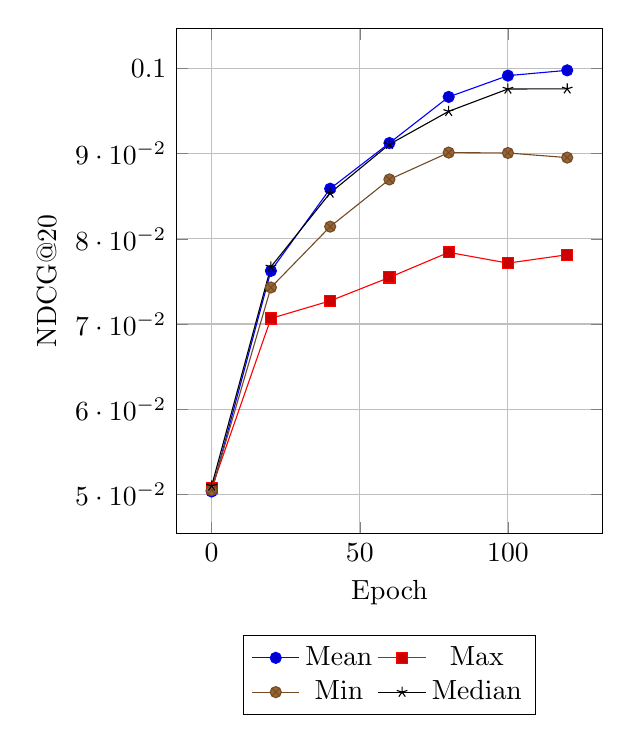
\begin{tikzpicture}
        \begin{axis}[
            xlabel=Epoch,
            ylabel=NDCG@20,
            height=8cm,
            width=7cm,
            grid=major,
            legend style={at={(0.5,-0.20)},
        anchor=north,legend columns=2}]
            
        \addplot plot coordinates{
        	(0,0.05035)
            (20,0.07624)
            (40,0.08588)
            (60,0.09124)
            (80,0.09665)
            (100,0.09915)
            (120,0.09977)
        };

		\addplot plot coordinates{
        	(0,0.05072)
            (20,0.07066)
            (40,0.07272)
            (60,0.07547)
            (80,0.07841)
            (100,0.07715)
            (120,0.07813)
        };

        \addplot plot coordinates{
        	(0,0.05051)
            (20,0.07429)
            (40,0.08143)
            (60,0.08697)
            (80,0.09012)
            (100,0.09007)
            (120,0.08953)
        };
        
        \addplot plot coordinates{
        	(0,0.051)
            (20,0.07671)
            (40,0.08538)
            (60,0.09109)
            (80,0.09496)
            (100,0.09758)
            (120,0.0976)
        };

        \legend{Mean,Max,Min,Median}
        \end{axis}
    \end{tikzpicture}
    \caption{Effect of aggregation functions on the YelpNC dataset for NDCG@20.}
    \label{fig:aggregation_effect}
\end{figure}


In \Cref{fig:aggregation_effect} we see the graph over how the choice of aggregation affects the CSGCN-IS model.
What we see is that taking the mean provides the best results, followed by the median.
In the bottom we have the simple solution of simply taking the lowest or highest score across the contexts.\\
This supports our previous assumption that while a single item might score high or low in one context, it does not necessarily mean that it is a good recommendation overall, which is better captured through the mean and median aggregations.\\
While the results are only shown for NDCG@20 for this dataset, they have proven consistent across all the metrics.
\\\\
To test whether context and side-information actually increase the performance of our model in a non-context specific setting, we run one of our proposed methods, CSGCN-ADJ, using different inputs for the datasets YelpNC and ML1M and measure the performances with NDCG@20.
First of all, our method is run with both side-information and context. 
Then we remove side-information, followed by removing context and finally we remove both context and side-information.
\begin{figure}
    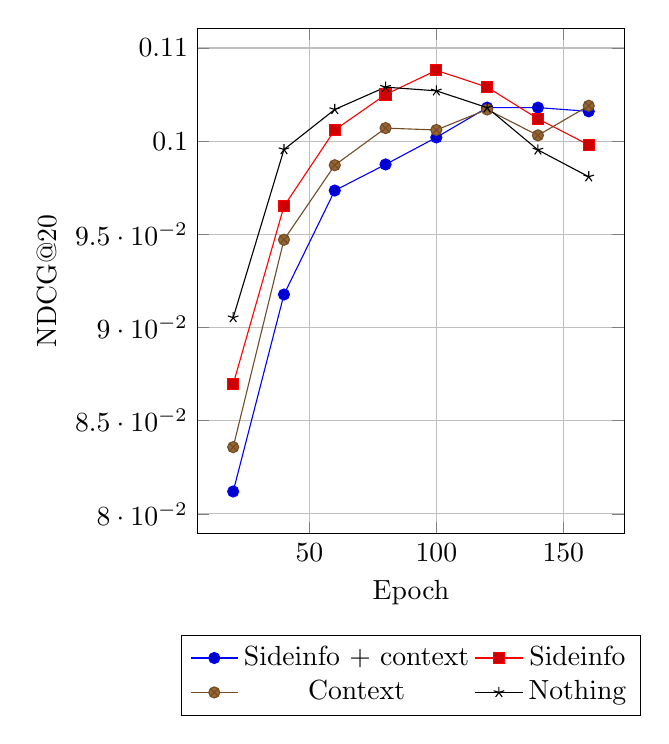
\begin{tikzpicture}
        \begin{axis}[
            xlabel=Epoch,
            ylabel=NDCG@20,
            height=8cm,
            width=7cm,
            grid=major,
            legend style={at={(0.5,-0.20)},
        anchor=north,legend columns=2}]
            
        \addplot plot coordinates{
            (20,8.120e-02)
            (40,9.177e-02)
            (60,9.735e-02)
            (80,9.875e-02)
            (100,1.002e-01)
            (120,1.018e-01)
            (140,1.018e-01)
            (160,1.016e-01)
        };

        \addplot plot coordinates {
            (20,8.696e-02)
            (40,9.651e-02)
            (60,1.006e-01)
            (80,1.025e-01)
            (100,1.038e-01)
            (120,1.029e-01)
            (140,1.012e-01)
            (160,9.98e-02)
        };

        \addplot plot coordinates {
            (20,8.358e-02)
            (40,9.471e-02)
            (60,9.871e-02)
            (80,1.007e-01)
            (100,1.006e-01)
            (120,1.017e-01)
            (140,1.0031e-01)
            (160,1.019e-01)
        };

        \addplot plot coordinates {
            (20,9.053e-02)
            (40,9.955e-02)
            (60,1.017e-01)
            (80,1.029e-01)
            (100,1.027e-01)
            (120,1.018e-01)
            (140,9.953e-02)
            (160,9.809e-02)

        };
        \legend{Sideinfo + context,Sideinfo,Context,Nothing}
        \end{axis}
    \end{tikzpicture}
    \caption{The performance on NDCG@20 of our model on the YelpNC dataset with different types of input.}
    \label{fig:ablation_study_1}
\end{figure}
On \Cref{fig:ablation_study_1} we see the performance on NDCG@20 of CSGCN-ADJ with different input.
We see that the more input the model receives, the longer it takes to converge to its best performance.
Overall, the performance does not change drastically with the different types of input.
Having only side-information as input achieves the best performance, but it is only marginally better than not having side-information and context at all.
Having both context and side-information actually degrades performance slightly, compared to just having side-information as the input, and having just context as input also does not give much better results.
To conclude from the study on the YelpNC dataset, the usage of context is not able to provide better recommendations in a non-context specific setting for the NDCG metric.
Side-information, however, performs the best on this metric on this dataset, which suggests that side-information in CSGCN-ADJ is able to slightly improve results compared to having no extra input.

\begin{figure}
    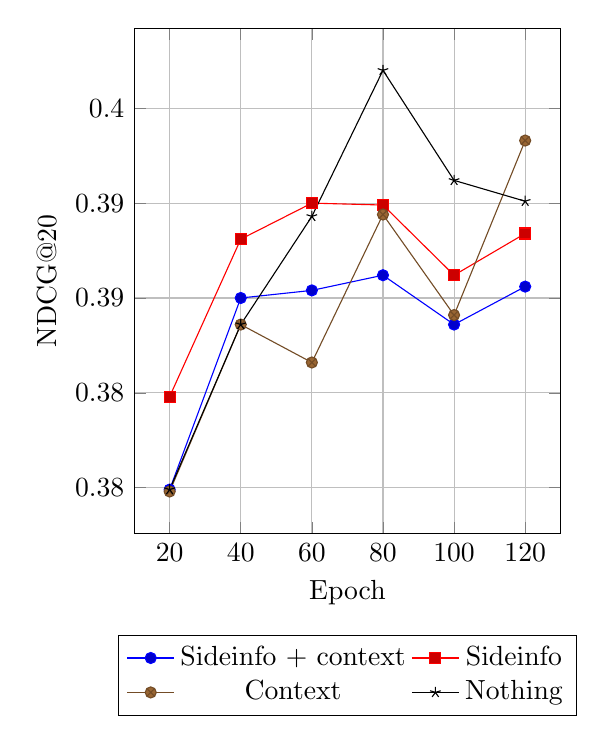
\begin{tikzpicture}
        \begin{axis}[
            xlabel=Epoch,
            ylabel=NDCG@20,
            height=8cm,
            width=7cm,
            grid=major,
            legend style={at={(0.5,-0.20)},
        anchor=north,legend columns=2}]
            
        \addplot plot coordinates{
            (20,0.3749)
            (40,0.3850)
            (60,0.3854)
            (80,0.3862)
            (100,0.3836)
            (120,0.3856)
        };

        \addplot plot coordinates {
            (20,0.3798)
            (40,0.3881)
            (60,0.3900)
            (80,0.3899)
            (100,0.3862)
            (120,0.3884)
        };

        \addplot plot coordinates {
            (20,0.3748)
            (40,0.3836)
            (60,0.3816)
            (80,0.3894)
            (100,0.3841)
            (120,0.3933)
        };

        \addplot plot coordinates {
            (20,0.3749)
            (40,0.3836)
            (60,0.3893)
            (80,0.3970)
            (100,0.3912)
            (120,0.3901)
        };
        \legend{Sideinfo + context,Sideinfo,Context,Nothing}
        \end{axis}
    \end{tikzpicture}
    \caption{The performance on NDCG@20 of our model on the ML1M dataset with different types of input.}
    \label{fig:ablation_study_2}
\end{figure}
On \Cref{fig:ablation_study_2} the NDGC@20 results of ML1M are shown for CSGCN-ADJ with different types of input. 
For this dataset, the model that uses neither the context nor side-information for the input is actually the best performing version.
Side-information and context is not able to improve the performance of the model on ML1M in a non-context specific setting.
Since both \Cref{fig:ablation_study_1,fig:ablation_study_2} show that the model is worse with context included, we can conclude that context does not increase the performance of CSGCN-ADJ in a non-context specific setting.
Side-information, however, should be able to increase performance of the model in a non-context specific setting, but in this case the side-information does not provide any additional collaborative signal.

\subsection{Performance Comparison (RQ3)}
To answer whether side-information improves the results for context-aware recommendations, we performed an ablation study with multiple ways of considering the side-information.
